\documentclass[a4paper,12pt]{scrartcl}
\usepackage[utf8x]{inputenc}
\usepackage[T1]{fontenc} % avec T1 comme option  d'encodage c'est ben mieux, surtout pour taper du français.
%\usepackage{lmodern,textcomp} % fortement conseillé pour les pdf. On peut mettre autre chose : kpfonts, fourier,...
\usepackage[french]{babel} %Sans ça les guillemets, amarchpo
\usepackage{amsmath}
\usepackage{multicol}
\usepackage{amssymb}
\usepackage{tkz-tab}
\usepackage{exercice_sheet}

%\trait
%\section*{}
%\exo{}
%\question{}
%\subquestion{}

\date{}


% Title Page
\title{Devoir maison 1 corrigé}

\author{Mathématiques}

\begin{document}

\maketitle

\exo{Racines carrées}

Simplifier les racines suivantes.

\question{}
$\sqrt{300} = \sqrt{3 \times 100} = 10 \sqrt{3}$

\question{}
$\sqrt{180} = \sqrt{5 \times 36} = 6 \sqrt{5}$

\question{}
$\sqrt{192} = \sqrt{3 \times 64} = 8 \sqrt{3}$

\question{}
$\sqrt{3528} = \sqrt{2 \times 1764} = 42 \sqrt{2}$

\exo{Factorisations}

Factoriser puis réduire les expressions suivantes.

\question{}
$x^2 + 2x = x(x+2)$

\question{}
$4x^2 + 8x + 4 = 4(x^2 + 2x + 1) = 4(x+1)^2$

\question{}
$9x^2 - 144 = 9(x^2 - 16) = 9(x+4)(x-4)$

\question{}
$12x^2 - 24x + 12 = 12(x^2 - 2x + 1) = 12(x-1)^2$

\exo{Polynômes du 2\textsuperscript{nd} degré}

Pour chacun de ces polynômes, trouver les racines dans $\mathbb{R}$, les factoriser et donner le tableau de signe.

Rappel : pour un polynôme du second degré de la forme $P(x) = ax^2 + bx + c$, $\Delta = b^2 - 4ac$, si $\Delta > 0$, $x_1 = \dfrac{-b-\sqrt{\Delta}}{2a}$ $x_2 = \dfrac{-b+\sqrt{\Delta}}{2a}$.

On rappelle également qu'un polynôme dont les racines sont $x_1$ et $x_2$ se factorise sous la forme suivante : $P(x) = a(x-x_1)(x-x_2)$.

\question{}%***
$5x^2 + x - 6$

$\Delta = 1^2 - 4 \times 5 \times (-6) = 121$

$\sqrt{\Delta} = 11$

$$x_1 = \dfrac{-1-11}{10} = \dfrac{-6}{5}$$

$$x_2 = \dfrac{-1+11}{10} = 1$$

La forme factorisée est donc : $5 \left(x - 1\right)\left(x + \dfrac{6}{5} \right)$

Tableau de signe:

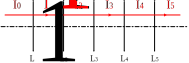
\includegraphics[width=0.5\textwidth]{pics/1.png}

\question{}%***
$-6x^2 + x + 7$

$\Delta = 1^2 - 4 \times (-6) \times 7 = 169$

$\sqrt{\Delta} = 13$

$$x_1 = \dfrac{-1-13}{-12} = \dfrac{7}{6}$$

$$x_2 = \dfrac{-1+13}{-12} = -1$$

La forme factorisée est donc : $-6 \left(x + 1\right)\left(x - \dfrac{7}{6} \right)$

Tableau de signe:

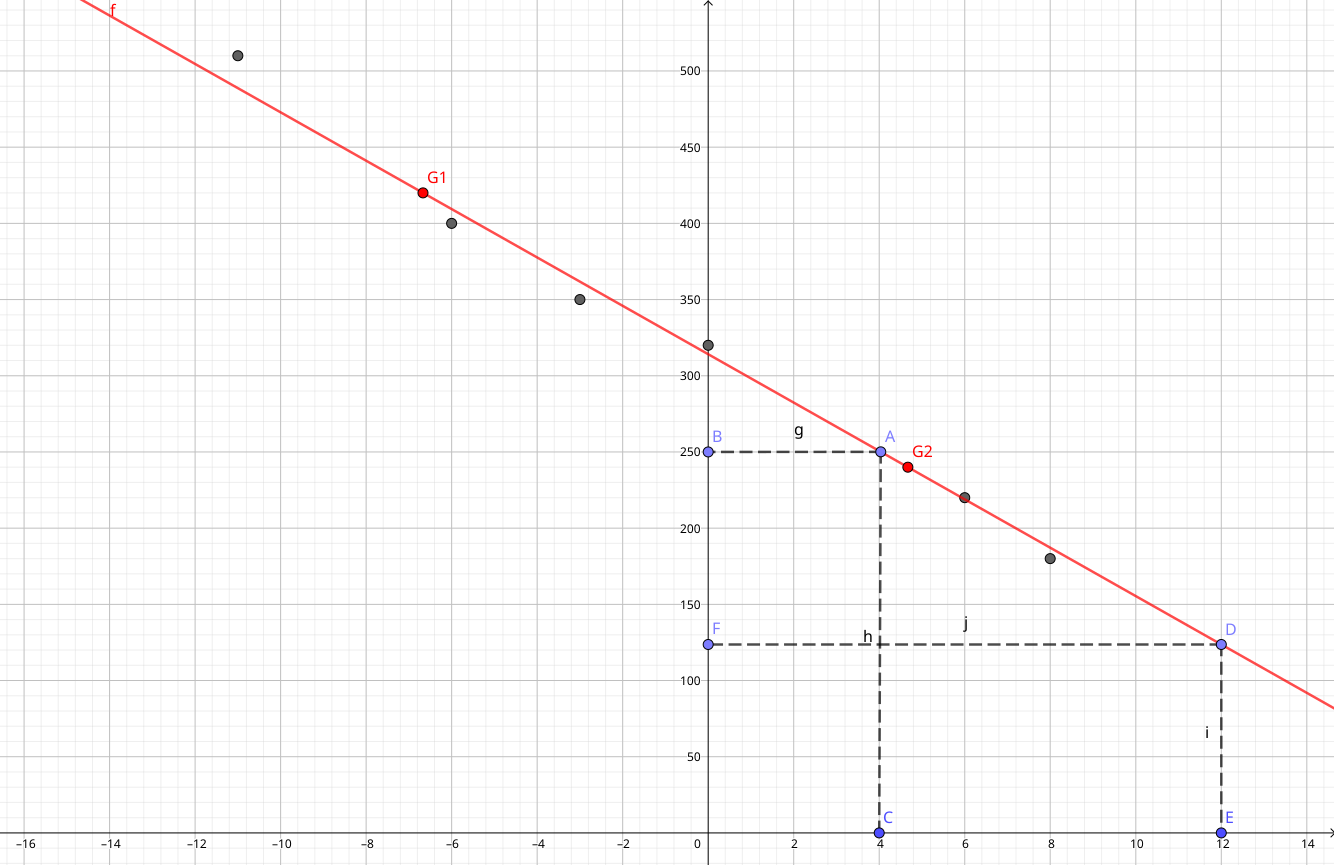
\includegraphics[width=0.5\textwidth]{pics/2.png}

\question{}%***
$2x^2 + x - 3$

$\Delta = 1^2 - 4 \times 2 \times (-3) = 25$

$\sqrt{\Delta} = 5$

$$x_1 = \dfrac{-1-5}{4} = -\dfrac{3}{2}$$

$$x_2 = \dfrac{-1+5}{4} = 1$$

La forme factorisée est donc : $2 \left(x - 1\right)\left(x + \dfrac{3}{2} \right)$

Tableau de signe:

\includegraphics[width=0.5\textwidth]{pics/3.png}

\question{}%***
$-3x^2 -5x +2$

$\Delta = (-5)^2 - 4 \times (-3) \times 2 = 49$

$\sqrt{\Delta} = 7$

$$x_1 = \dfrac{5-7}{-6} = \dfrac{1}{3}$$

$$x_2 = \dfrac{5+7}{-6} = -2$$

La forme factorisée est donc : $-3 \left(x + 2\right)\left(x - \dfrac{1}{3} \right)$

Tableau de signe:

\includegraphics[width=0.5\textwidth]{pics/4.png}

\exo{Systèmes de 2 équations à 2 inconnues}

\question{}
$$
\begin{cases} 
a+b &= 0 \\
a-b &= 6
\end{cases}
$$

On additionne la 1\textsuperscript{re} ligne et la 2\textsuperscript{ème} afin d'éliminer l'inconnue $b$. On obtient:

$2a = 6 \Leftrightarrow a = 3$

En remplaçant $a$ par sa valeur dans la 1\textsuperscript{re} équation, on obtient: $3 + b=6 \Leftrightarrow b = -3$. 

On obtient donc $a = 3$ et $b = -3$.

\question{}
$$
\begin{cases} 
2f+3g &= 8 \\
-f+2g &= 3
\end{cases}
$$

On multiplie la 2\textsuperscript{ème} ligne par 2, de façon à éliminer l'inconnue $f$ en additionnant les 2 lignes. On obtient donc :

$$
\begin{cases} 
2f+3g &= 8 \\
-2f+4g &= 6
\end{cases}
$$

On additionne la 1\textsuperscript{re} ligne et la 2\textsuperscript{ème} afin d'éliminer l'inconnue $f$. On obtient:

$7g = 14 \Leftrightarrow g = 2$

En remplaçant $g$ par sa valeur dans la 2\textsuperscript{ème} équation, on obtient: $-f + 2 \times 2 = 3 \Leftrightarrow f = 1$. 

On obtient donc $f = 1$ et $g = 2$.

\question{}
$$
\begin{cases} 
3y+z &= 9 \\
\dfrac{z}{2} + 2y &= 8
\end{cases}
$$

On remarque que dans la 2\textsuperscript{ème} équation, les inconnues ne sont pas ordonnées. On réécrit donc le système:

$$
\begin{cases} 
3y+z &= 9 \\
2y + \dfrac{1}{2} z &= 8
\end{cases}
$$

En multipliant la 2\textsuperscript{ème} ligne par -2 on pourra éliminer l'inconnue $z$ par addition:
 
$$
\begin{cases} 
3y+z &= 9 \\
-4y - z &= -16
\end{cases}
$$

On additionne la 1\textsuperscript{re} ligne et la 2\textsuperscript{ème} afin d'éliminer l'inconnue $z$. On obtient:

$-y = -7 \Leftrightarrow y = 7$

En remplaçant $y$ par sa valeur dans la 1\textsuperscript{re} équation, on obtient: $3 \times 7 + z=9 \Leftrightarrow z = -12$. 

On obtient donc $y = 7$ et $z = -12$.

\question{}
Dans une étable peuplée uniquement de poules et de vaches, il y a 38 têtes et 120 pattes. Combien y'a-t-il de poules, combien y'a-t-il de vaches?

On rappelle si besoin que les poules ont 2 pattes et les vaches en ont 4. 

Également, chaque animal a une tête, et une seule.

On appelle $p$ le nombre de poules et $v$ le nombre de vaches. 

Dans l'énoncé, l'information relative au nombre total de têtes permet d'écrire l'équation $p+v = 38$.

L'information relative au nombre de pattes permet d'écrire $2p + 4v = 120$. 

On peut donc écrire le système suivant:

$$
\begin{cases} 
p+v &= 38 \\
2p + 4v &= 120
\end{cases}
$$

Le système se résout de la même façon que dans les questions précédentes:

On multiplie la 1\textsuperscript{re} ligne par -2:

$$
\begin{cases} 
-2p + -2v &= -76 \\
2p + 4v &= 120
\end{cases}
$$

En additionnant les 2 lignes, on obtient: $2v = 44 \Leftrightarrow v = 22$.

En remplaçant $v$ par sa valeur dans la 1\textsuperscript{re} équation, on obtient : $p+22 = 38 \Leftrightarrow p = 16$.

On a donc $p = 16$ et $v = 22$. 

Il y a donc 16 poules et 22 vaches dans l'étable. 

\exo{Statistiques}

On a mesuré les tailles en cm des personnes dans un groupe de 16 personnes. Voici les résultats:

140, 141, 148, 153, 156, 157, 158, 164, 171, 181, 182, 190, 191, 195, 196, 199

Indiquer:

\question{L'étendue}

L'étendue est la différence entre la plus grande valeur et la plus petite. 

Ici: $199 - 140 = 59 \mbox{cm}$.

\question{La moyenne}

On additionne toutes les valeurs et on divise par l'effectif.

$\dfrac{140 + 141 + 148 + \ldots + 199}{16} = 170.125 \mbox{cm}$ que l'on peut arrondir à 170 cm.

\question{La médiane}

L'effectif est de 16, la médiane est donc la moyenne entre la 8\textsuperscript{ème} et la 9\textsuperscript{ème} valeur: $\dfrac{164+171}{2} = 167.5 \mbox{cm}$

\question{Le premier et le troisième quartile}

$16 \times \dfrac{1}{4} = 4$. $Q_1$ est donc la 4\textsuperscript{ème} valeur de la série rangée dans l'ordre croissant. 

$Q_1 = 153\mbox{cm}$.

$16 \times \dfrac{3}{4} = 12$. $Q_3$ est donc la 12\textsuperscript{ème} valeur de la série rangée dans l'ordre croissant. 

$Q_3 = 190\mbox{cm}$.


\trait

\end{document}
